\subsection{Examples of games Population of small agents}




The following are some examples of games with small number of agents. 
We implement the rock-paper-scissors game. This game has only one population with three strategies, denoted $x = [x_1, x_2, x_3]^\top$. The fitness function is defined as $F(x)=Ax$, where A is equal to 
\begin{equation}
  A = \begin{pmatrix}
  0  & -1 &  1 \\
  1  &  0 & -1 \\
  -1 &  1 & 0
  \end{pmatrix}
\end{equation}

We implement four revision protocols, namely, proportional imitation, comparison to average, pairwise comparison, and logit choice. Fig. \ref{fig:finite1} to \ref{fig:finite4} show the evolution of the society with each revision protocol.

Simulations are made with $200$ agents and 10000 iterations.
The evolution might take place in days, months, years.




\begin{figure}
  \centering
  \begin{subfigure}[b]{0.45\textwidth}
	  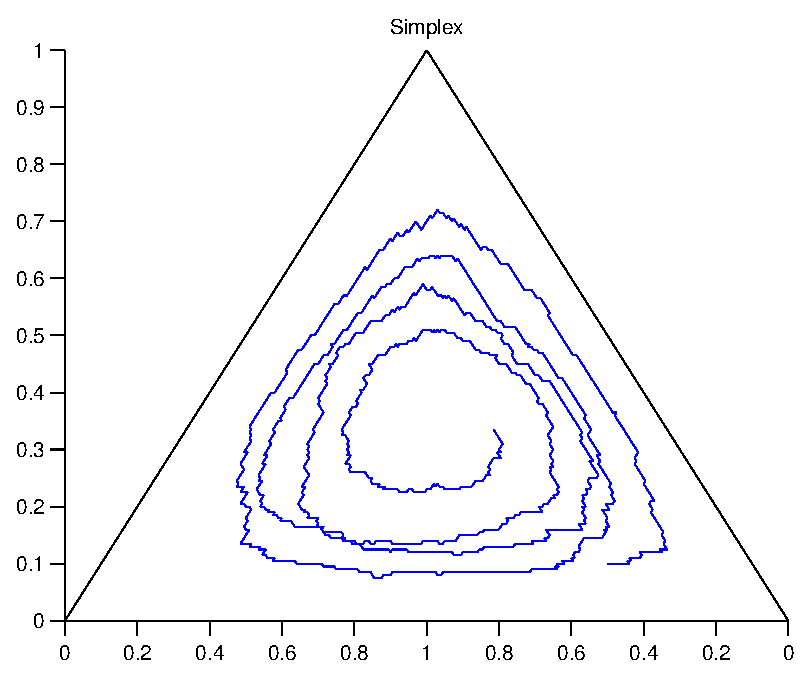
\includegraphics[width=\textwidth]{./images/test_finite_proportional_imitation.eps}
	  \caption{Simplex.}
	  \label{fig:finite1_simplex}
  \end{subfigure}
  ~ 
  \begin{subfigure}[b]{0.45\textwidth}
	  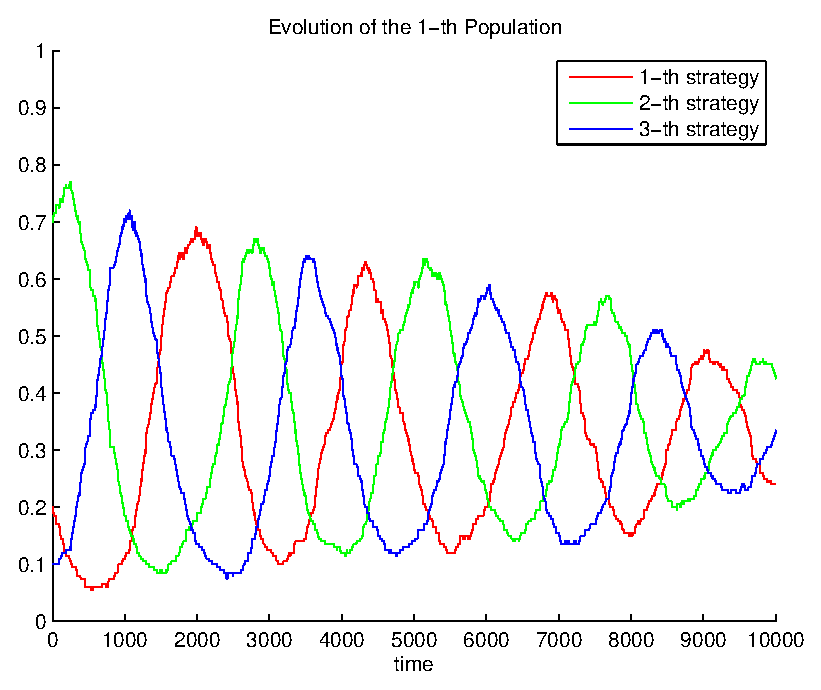
\includegraphics[width=\textwidth]{./images/test_finite_proportional_imitation_ev.eps}
	  \caption{Evolution of the strategies in time.}
	  \label{fig:finite1_ev}
  \end{subfigure}
  \caption{Rock-paper-scissors game with proportional imitation revision protocol (Replicator dynamics with large number of agents).}
  \label{fig:finite1}
\end{figure}


\begin{figure}
  \centering
  \begin{subfigure}[b]{0.45\textwidth}
	  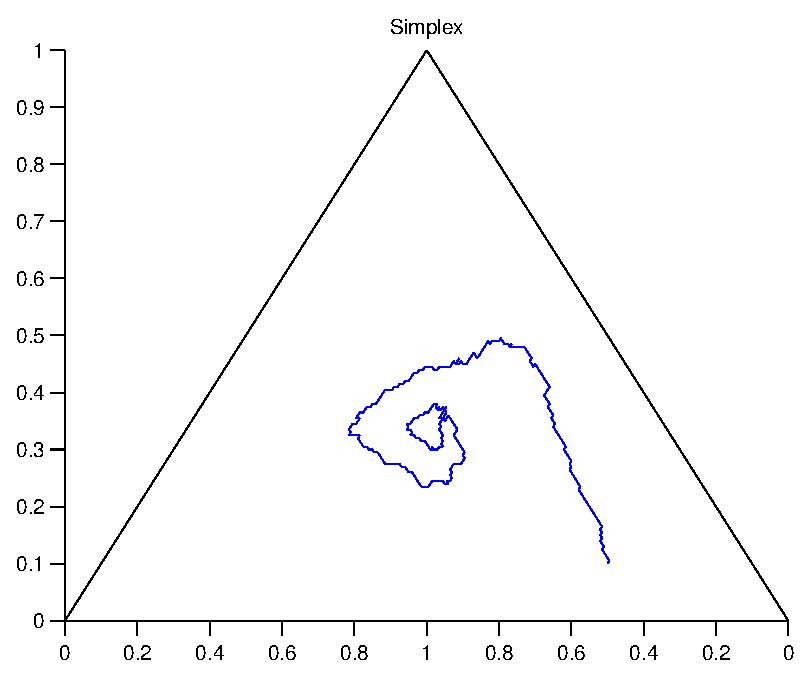
\includegraphics[width=\textwidth]{./images/test_finite_comparison2average.eps}
	  \caption{Simplex.}
	  \label{fig:finite2_simplex}
  \end{subfigure}
  ~ 
  \begin{subfigure}[b]{0.45\textwidth}
	  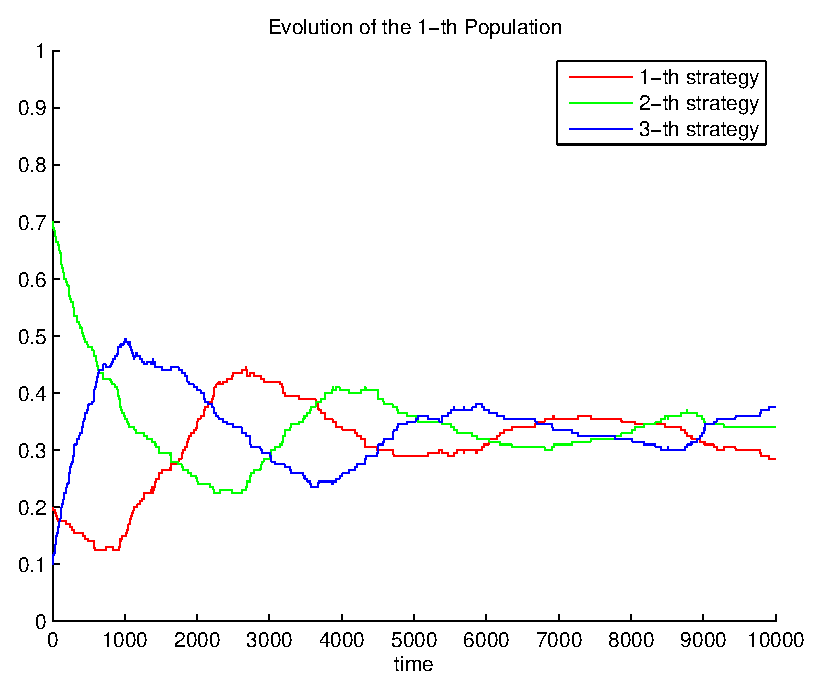
\includegraphics[width=\textwidth]{./images/test_finite_comparison2average_ev.eps}
	  \caption{Evolution of the strategies in time.}
	  \label{fig:finite2_ev}
  \end{subfigure}
  \caption{Rock-paper-scissors game with comparison to average revision protocol (BNN dynamics with large number of agents).}
  \label{fig:finite2}
\end{figure}


\begin{figure}
  \centering
  \begin{subfigure}[b]{0.45\textwidth}
	  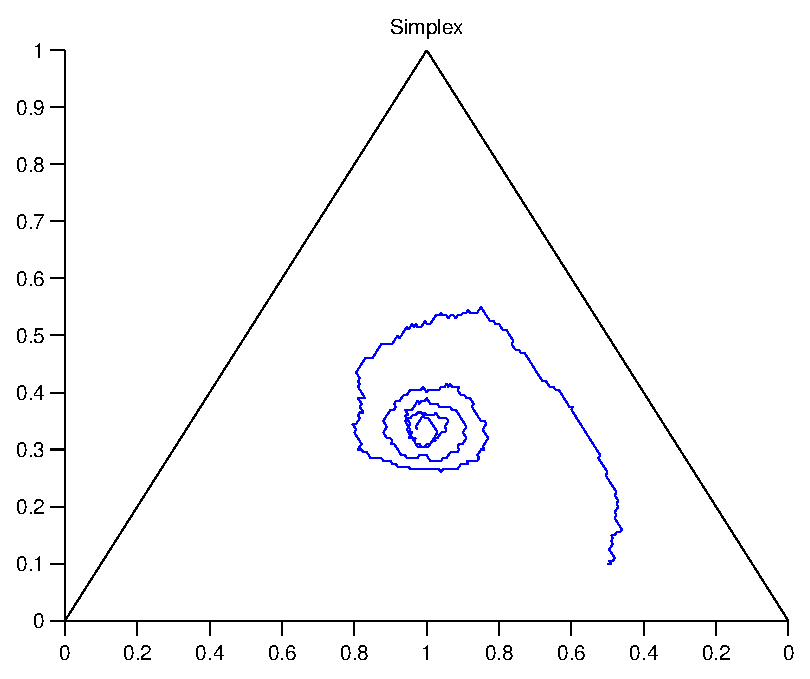
\includegraphics[width=\textwidth]{./images/test_finite_pairwise_comparison.eps}
	  \caption{Simplex.}
	  \label{fig:finite3_simplex}
  \end{subfigure}
  ~ 
  \begin{subfigure}[b]{0.45\textwidth}
	  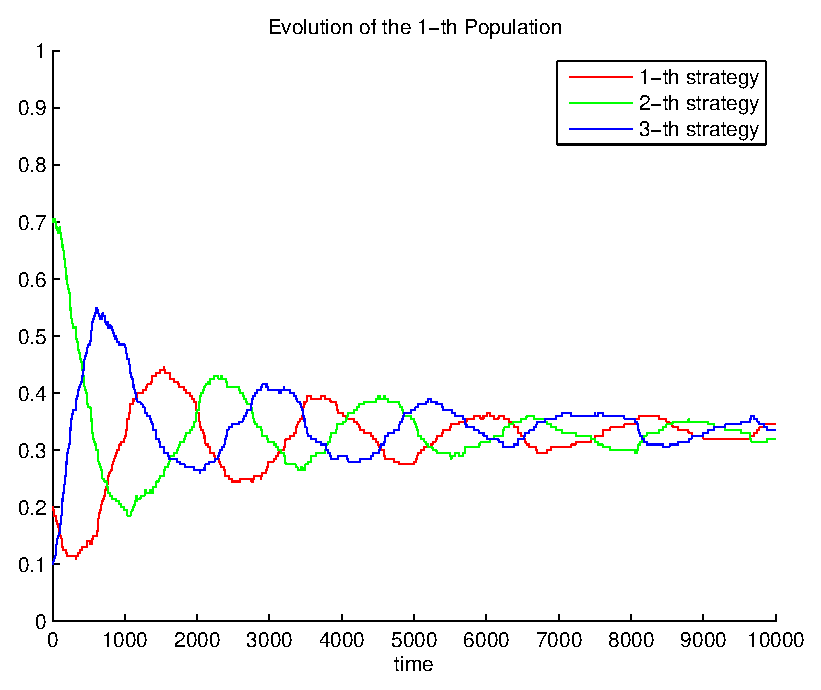
\includegraphics[width=\textwidth]{./images/test_finite_pairwise_comparison_ev.eps}
	  \caption{Evolution of the strategies in time.}
	  \label{fig:finite3_ev}
  \end{subfigure}
  \caption{Rock-paper-scissors game with pairwise comparison revision protocol (Smith dynamics with large number of agents).}
  \label{fig:finite3}
\end{figure}


\begin{figure}
  \centering
  \begin{subfigure}[b]{0.45\textwidth}
	  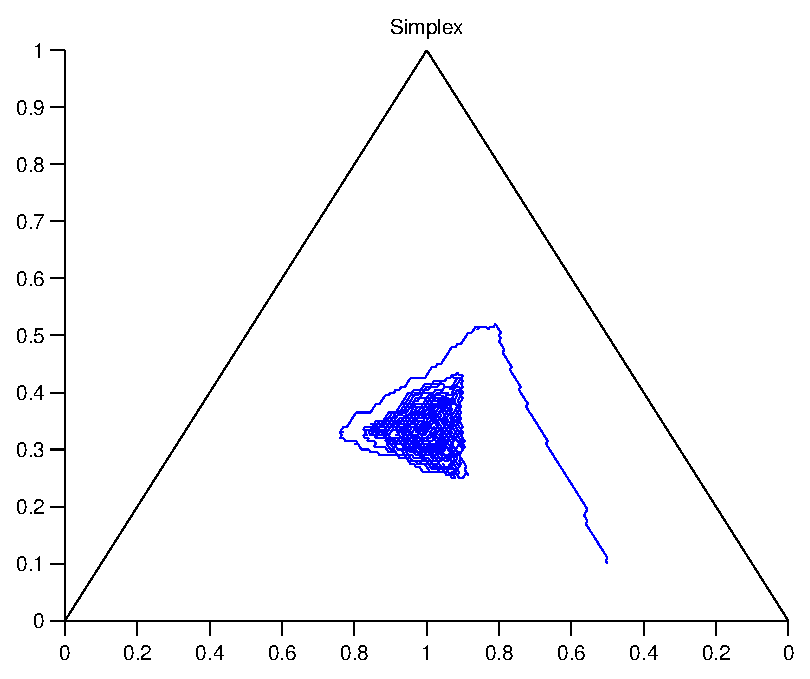
\includegraphics[width=\textwidth]{./images/test_finite_logit_choice.eps}
	  \caption{Simplex.}
	  \label{fig:finite4_simplex}
  \end{subfigure}
  ~ 
  \begin{subfigure}[b]{0.45\textwidth}
	  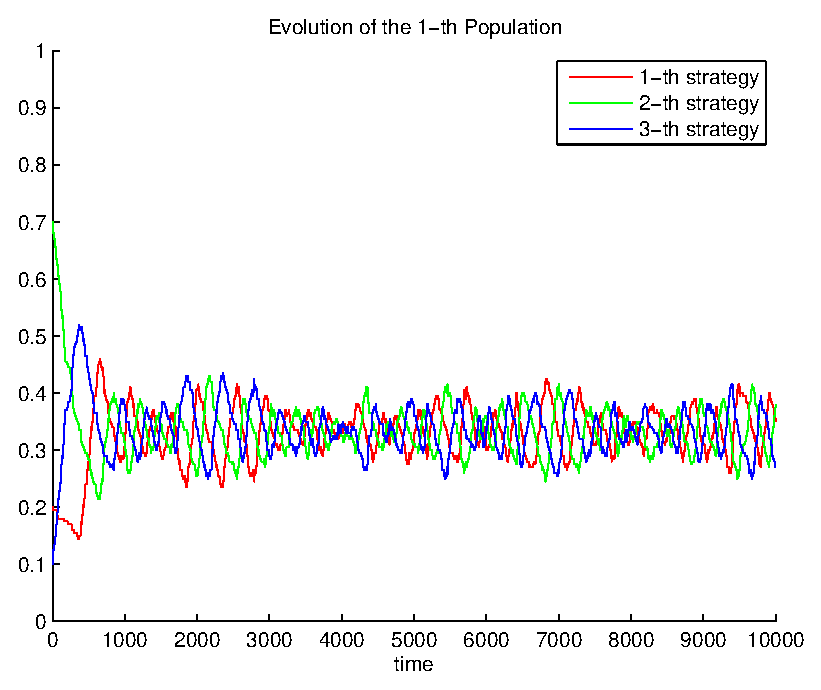
\includegraphics[width=\textwidth]{./images/test_finite_logit_choice_ev.eps}
	  \caption{Evolution of the strategies in time.}
	  \label{fig:finite4_ev}
  \end{subfigure}
  \caption{Rock-paper-scissors game with logit choice revision protocol ( dynamics with large number of agents).}
  \label{fig:finite4}
\end{figure}




